\documentclass[11pt]{article}

\usepackage[margin=1in]{geometry}
\usepackage{amsmath,amssymb,amsfonts}
\usepackage{booktabs,multirow,array}
\usepackage{graphicx}
\usepackage{subcaption}
\usepackage{xcolor}
\usepackage{hyperref}
\usepackage{url}
\usepackage{tikz}
\usepackage{enumitem}
\usepackage{microtype}
\usepackage{placeins}
\usetikzlibrary{arrows.meta,positioning,shapes.geometric,fit}

\hypersetup{
  colorlinks=true,
  linkcolor=blue!55!black,
  citecolor=blue!55!black,
  urlcolor=blue!55!black
}

\graphicspath{{./}}

\newcommand{\sympy}{SymPy}
\newcommand{\kan}{KAN}
\newcommand{\hyperkan}{HyperKAN}
\newcommand{\staticKAN}{Static KAN}
\newcommand{\mlp}{MLP}
\newcommand{\bce}{\operatorname{BCE}}
\newcommand{\huber}{\operatorname{Huber}}
\newcommand{\E}{\mathbb{E}}
\setlength{\emergencystretch}{2em}
\setlist[itemize]{topsep=3pt,itemsep=2pt,leftmargin=1.2em}
\setlist[enumerate]{topsep=3pt,itemsep=2pt,leftmargin=1.4em}

\tikzset{
  paperbox/.style={draw, rounded corners, align=center, inner sep=5pt, minimum height=0.75cm, font=\small},
  paperarrow/.style={-Latex, thick},
  paperlabel/.style={font=\footnotesize, align=center}
}

\title{\textbf{Scoped Actions Expose Compositional Failures in Verified Symbolic Rewrite Search}}
\author{Marcel\\Independent Researcher}
\date{}

\begin{document}
\maketitle

\begin{abstract}
We present a controlled mechanistic benchmark study of learned heuristics for formally verified symbolic rewrite search in algebraic reasoning. Our starting point is a global-action benchmark in which a model predicts one of six whole-expression \sympy{} rewrites (\texttt{expand}, \texttt{factor}, \texttt{cancel}, \texttt{apart}, \texttt{together}, \texttt{trigsimp}) toward an exact target form, and a search loop verifies success by executing those rewrites symbolically. On this benchmark, a \staticKAN{} head outperforms an \mlp{} baseline, while an initial goal-conditioned \hyperkan{} underperforms and only becomes competitive after reducing hypernetwork capacity. Exact graph mining of the benchmark reveals a deeper issue: whole-expression rewrite semantics make composition shallow, so apparent difficulty collapses under global transformations.

To address this, we introduce a scoped-action benchmark in which actions are pairs of the form $(u,o)$, where $u$ is a deterministic subtree location and $o$ is one of the original rewrite families. Guided scoped datasets validate that the end-to-end pipeline is trainable, but only a structural held-out-family probe produces real compositional pressure. On this probe, both \staticKAN{} and recovered \hyperkan{} solve seen families but fail completely on a held-out mixed composition family by default, revealing a root-action collapse failure mode. A simple inference-side localization bias substantially rescues \hyperkan{}, and a frontier-aware reranker improves held-out mixed-family beam solve rate further, indicating that early hidden-branch access is a key mechanism for compositional success. A lightweight Transformer-encoder diagnostic also fails by default on the held-out mixed family, suggesting that the failure is not confined to the original recurrent encoder. A deeper depth-7 expansion then exposes a clear failure boundary: the moderate-depth rescue does not carry over cleanly to deeper compositions. Additional bounded diagnostics show that learned frontier supervision and a frontier-head-only RL controller do not internalize this deeper transfer behavior.

These controlled results support four bounded conclusions. First, benchmark semantics and action granularity can dominate apparent reasoning difficulty in this verified symbolic search setting. Second, supervised validation loss is an unreliable proxy for search performance. Third, moderate compositional gains can be obtained through inference-time frontier shaping, but current training objectives do not internalize that behavior. Fourth, the current mechanism has a measurable depth boundary rather than scaling smoothly with chain length. We do not claim that \hyperkan{} wins universally, that root-collapse is universal across neural architectures, or that the resulting system solves symbolic reasoning.
\end{abstract}

\section{Introduction}

A recurring failure mode in neural-symbolic reasoning is to confuse cosmetic algebraic complexity with actual multi-step reasoning depth. Expressions can look complicated while remaining one rewrite away from a target under a sufficiently strong global action vocabulary. For this reason, benchmark design is inseparable from model evaluation: if the rewrite graph is shallow, apparent reasoning gains may be artifacts of local ranking rather than evidence of long-horizon symbolic control.

This paper studies that problem in a deliberately formal setting. We train policy/value models for symbolic rewrite search where every state transition is executed by \sympy{} and every final success condition is exactly verifiable. The original benchmark uses a small global action space consisting of six whole-expression \sympy{} rewrites. Within that setting, a \staticKAN{} policy head outperforms an \mlp{} baseline, while an initial goal-conditioned \hyperkan{} underperforms. After reducing hypernetwork capacity, \hyperkan{} nearly matches \staticKAN{} on the shallow global benchmark, but detailed analysis shows that supervised validation loss and verified search performance diverge sharply.

At that point, the project becomes a benchmark-design problem as much as a modeling problem. Exact graph mining shows that global whole-expression rewrites admit isolated depth-2 and depth-3 ladders but do not yield robust depth-4+ compositional families at useful density. This motivates a benchmark redesign around scoped actions: instead of predicting only which rewrite to apply, the model predicts where in the expression to apply it.

The scoped reformulation immediately validates the pipeline, but the first guided datasets are too templated to separate models. The first meaningful benchmark is a structural held-out-family probe: models train on three single-block families and are evaluated on a mixed composition family never seen in training. This probe is non-saturated and exposes a concrete failure mode: both \staticKAN{} and recovered \hyperkan{} collapse to root-level whole-expression actions instead of selecting local subgoals. Inference-time localization and frontier shaping partially rescue \hyperkan{} on this moderate-depth probe, but a deeper depth-7 expansion shows that the rescue has a clear boundary.

The paper makes four contributions:
\begin{enumerate}
  \item A verified symbolic rewrite benchmark analysis showing that global whole-expression semantics produce shallow composition even when isolated ladders exist.
  \item A scoped-action benchmark formulation with deterministic subtree sites and grouped \texttt{Add} slices that makes compositional failures visible.
  \item A structural held-out-family probe demonstrating that compositional generalization can fail completely despite success on seen families.
  \item A mechanism study showing that inference-time frontier shaping can rescue moderate-depth compositional performance by increasing early hidden-branch access, while current training-time fixes, learned frontier supervision, and a bounded frontier-head-only RL controller fail to internalize that behavior for deeper transfer.
\end{enumerate}

The intended claim is deliberately modest. This is a controlled benchmark-and-mechanism paper, not a universal theorem about neural symbolic models, not a claim that \hyperkan{} universally dominates \mlp{} or \staticKAN{}, and not a claim that symbolic reasoning has been solved. The benchmark is intentionally controlled so that action granularity, search, and model inductive bias can be studied under exact symbolic verification.

\section{Related Work}

This work sits at the intersection of symbolic computation, neural-guided formal search, and benchmark design for compositional reasoning. On the symbolic side, \sympy{} provides the executable rewrite substrate and exact target-form verification used throughout our experiments \cite{meurer2017sympy}. On the neural-guided search side, our setting is closer in spirit to learned heuristic guidance for formal reasoning than to pure one-step classification: the phenomenon of interest is how model scores interact with search frontier management under exact symbolic execution \cite{loos2017deep,polu2020gen}. On the architecture side, \kan{}s provide a structured spline-based alternative to dense policy heads, while \hyperkan{} asks whether goal-conditioned spline routing yields a useful inductive bias for symbolic rewrite control \cite{liu2024kan}. Finally, our emphasis on benchmark semantics is aligned with work arguing that the structure of a benchmark can dominate the difficulty it appears to measure \cite{chollet2019measure,trinh2024alphageometry}.

Our contribution differs from these lines in two ways. First, we show that whole-expression rewrite semantics can make a formally verified algebra benchmark compositionally shallow even when local ladders exist. Second, we expose a concrete search-control failure mode --- root-collapse --- on a scoped held-out-family probe, then analyze both the rescue mechanism and its failure boundary.

\section{Problem Setting}

We study goal-directed symbolic rewriting under exact verification. Each example consists of a current symbolic state $S$, an exact target form $G$, and a search procedure that executes candidate rewrites and checks whether the target has been reached. The model predicts actions conditioned on $(S,G)$. During inference, the model is embedded inside a beam-search loop. Search expands candidate states by applying model-scored actions, \sympy{} executes the corresponding rewrite, and exact matching against the target form determines success.

The crucial design choice is the action semantics.

\subsection{Global actions}

The original benchmark uses six whole-expression actions:
\[
\mathcal{O}=\{\texttt{expand},\texttt{factor},\texttt{cancel},\texttt{apart},\texttt{together},\texttt{trigsimp}\}.
\]
These actions are expressive and easy to verify, but they act globally. A single rewrite can often collapse multiple latent subproblems at once.

\subsection{Scoped actions}

The scoped benchmark keeps the same operator families but changes the granularity of control. Actions are represented as
\[
a=(u,o),
\]
where $u$ is a deterministic site identifier and $o\in\mathcal{O}$ is one of the rewrite types above. The scoped site model includes subtree path sites such as \texttt{expr@root}, \texttt{expr@1}, \texttt{numerator@1}, and \texttt{denominator@1}, plus grouped \texttt{Add} slices such as \texttt{add\_slice@root[0:2]}. This changes the task from predicting only what rewrite to apply to predicting both where and what.

\begin{figure}[t]
\centering
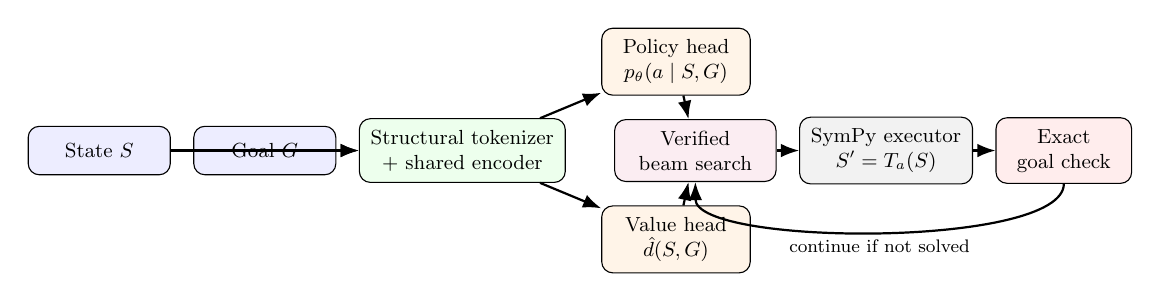
\begin{tikzpicture}[node distance=0.55cm and 0.35cm, transform shape, scale=0.82]
  \node[paperbox, fill=blue!7, minimum width=2.2cm] (state) {State $S$};
  \node[paperbox, fill=blue!7, minimum width=2.2cm, right=of state] (goal) {Goal $G$};
  \node[paperbox, fill=green!7, minimum width=2.8cm, right=of goal] (enc) {Structural tokenizer\\+ shared encoder};
  \node[paperbox, fill=orange!9, minimum width=2.3cm, above right=0.35cm and 0.55cm of enc] (policy) {Policy head\\$p_\theta(a\mid S,G)$};
  \node[paperbox, fill=orange!9, minimum width=2.3cm, below right=0.35cm and 0.55cm of enc] (value) {Value head\\$\hat d(S,G)$};
  \node[paperbox, fill=purple!7, minimum width=2.5cm, right=0.75cm of enc] (beam) {Verified\\beam search};
  \node[paperbox, fill=gray!10, minimum width=2.4cm, right=of beam] (sympy) {\sympy{} executor\\$S'=T_a(S)$};
  \node[paperbox, fill=red!7, minimum width=2.1cm, right=of sympy] (check) {Exact\\goal check};

  \draw[paperarrow] (state) -- (enc);
  \draw[paperarrow] (goal) -- (enc);
  \draw[paperarrow] (enc) -- (policy);
  \draw[paperarrow] (enc) -- (value);
  \draw[paperarrow] (policy) -- (beam);
  \draw[paperarrow] (value) -- (beam);
  \draw[paperarrow] (beam) -- (sympy);
  \draw[paperarrow] (sympy) -- (check);
  \draw[paperarrow] (check.south) .. controls +(0,-1.0) and +(0,-1.0) .. node[paperlabel, below] {continue if not solved} (beam.south);
\end{tikzpicture}
\caption{Verified symbolic rewrite search loop. The model scores actions and progress, but every transition is executed symbolically and every success condition is exactly checked.}
\label{fig:system}
\end{figure}

\section{Notation, Models, and Inference}

Let the current symbolic state be $S$ and the exact target form be $G$. A rewrite environment defines transitions
\[
S' = T_a(S),
\]
where $a$ is a discrete action and $T_a$ is the corresponding \sympy{} rewrite when valid. Invalid transitions are discarded by the search procedure.

For each example we observe a pair $(S,G)$ and one of two supervision types: a set of shortest valid next actions $A^\star(S,G)$, or a guided single-path next action $a^\star(S,G)$. We define the shortest-path distance to goal under the benchmark semantics as
\[
d(S,G)=
\min_{\substack{k\ge 0,\; a_1,\ldots,a_k\\
T_{a_k}\circ\cdots\circ T_{a_1}(S)=G}} k,
\]
when a valid path exists within the search horizon.

All models share a structural tokenizer over symbolic expressions and a common encoder backbone. The current state and goal are encoded as
\[
z_S=E(S), \qquad z_G=E(G),
\]
and fused into
\[
h=[z_S;z_G;z_S-z_G;z_S\odot z_G],
\]
where $\odot$ is elementwise multiplication and $[\cdot;\cdot]$ denotes concatenation. A value head predicts the distance-to-goal estimate $\hat d=v(h)$. The policy head differs by model family.

\paragraph{MLP baseline.} The \mlp{} policy head maps $h$ directly to action logits with a small dense network.

\paragraph{Static KAN.} The \staticKAN{} head replaces a dense mapping with spline-based edge functions. Abstractly, each output logit is built from sums of one-dimensional nonlinear edge functions over hidden coordinates:
\[
y_j=\sum_i \phi_{ij}(x_i),
\]
where each $\phi_{ij}$ is represented by a learned spline or a mixture over spline templates.

\paragraph{HyperKAN.} \hyperkan{} is a goal-conditioned \kan{} in which a hypernetwork modulates the policy head using the goal embedding. Let $H(\cdot)$ denote the hypernetwork. It maps the goal representation to modulation parameters $m=H(z_G)$. For an edge function represented as a mixture over $K$ templates,
\[
\phi_{ij}(x_i\mid z_G)=\sum_{k=1}^{K} \alpha_{ij,k}(z_G)\,\psi_{ij,k}(x_i),
\]
where the coefficients $\alpha_{ij,k}(z_G)$ are produced by the hypernetwork and $\psi_{ij,k}$ are learned template functions.

In a later factorized site/op variant, flat action logits are decomposed as
\[
\ell(u,o)=\ell_{\mathrm{site}}(u)+\ell_{\mathrm{op}}(o),
\]
with auxiliary site and operator losses added during training. This variant improves seen-family efficiency but does not solve the held-out mixed family.

\begin{figure}[t]
\centering
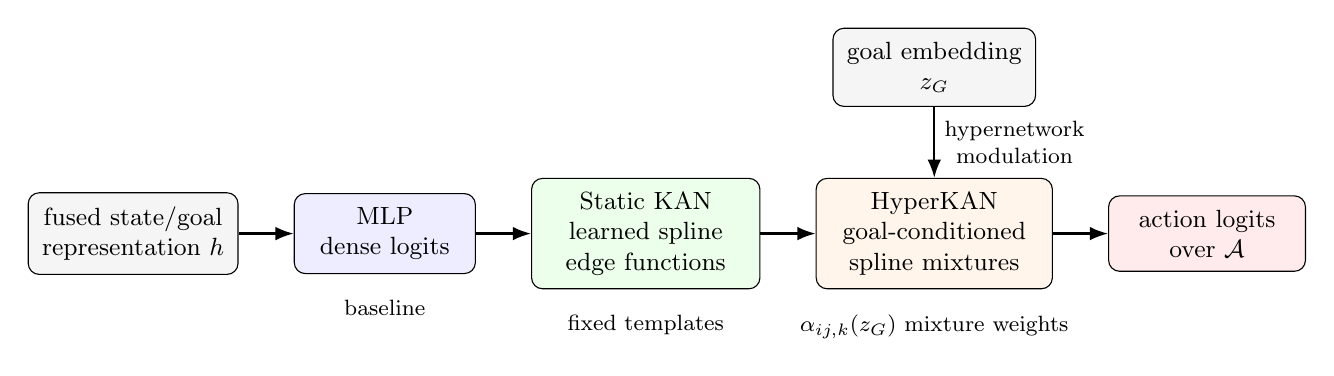
\begin{tikzpicture}[node distance=0.65cm and 0.7cm]
  \node[paperbox, fill=gray!8, minimum width=2.5cm] (h1) {fused state/goal\\representation $h$};
  \node[paperbox, fill=blue!7, minimum width=2.3cm, right=of h1] (mlp) {MLP\\dense logits};
  \node[paperbox, fill=green!8, minimum width=2.9cm, right=of mlp] (static) {Static KAN\\learned spline\\edge functions};
  \node[paperbox, fill=orange!8, minimum width=3.0cm, right=of static] (hyper) {HyperKAN\\goal-conditioned\\spline mixtures};
  \node[paperbox, fill=gray!8, minimum width=2.5cm, above=0.9cm of hyper] (zg) {goal embedding\\$z_G$};
  \node[paperbox, fill=red!8, minimum width=2.5cm, right=of hyper] (logits) {action logits\\over $\mathcal{A}$};

  \draw[paperarrow] (h1) -- (mlp);
  \draw[paperarrow] (mlp) -- (static);
  \draw[paperarrow] (static) -- (hyper);
  \draw[paperarrow] (hyper) -- (logits);
  \draw[paperarrow] (zg) -- node[paperlabel, right] {hypernetwork\\modulation} (hyper);

  \node[paperlabel, below=0.2cm of mlp] {baseline};
  \node[paperlabel, below=0.2cm of static] {fixed templates};
  \node[paperlabel, below=0.2cm of hyper] {$\alpha_{ij,k}(z_G)$ mixture weights};
\end{tikzpicture}
\caption{Policy-head comparison. The models share the same state/goal encoder and value head; the policy head changes from dense logits to static spline edge functions to goal-conditioned spline mixtures.}
\label{fig:policy-heads}
\end{figure}

Training combines an action loss and a value loss. For multi-label shortest-action supervision we use a binary cross-entropy style action loss over the valid shortest set $A^\star(S,G)$:
\[
\mathcal{L}_{\mathrm{act}}=\sum_{a\in\mathcal{A}} \bce\!\left(p_\theta(a\mid S,G),y_a\right),
\qquad y_a=\mathbf{1}[a\in A^\star(S,G)].
\]
For guided single-path scoped datasets, the target is a one-hot action $a^\star(S,G)$. Distance-to-goal is trained with a Huber regression loss $\mathcal{L}_{\mathrm{val}}=\huber(\hat d,d(S,G))$. The total loss is
\[
\mathcal{L}=\mathcal{L}_{\mathrm{act}}+\lambda_{\mathrm{val}}\mathcal{L}_{\mathrm{val}}+\mathcal{L}_{\mathrm{aux}},
\]
where $\mathcal{L}_{\mathrm{aux}}$ is zero for the base models and contains optional auxiliary terms in ablation branches, such as site/op supervision, root-avoidance penalties, or frontier-label losses.

At inference time, the model is embedded inside beam search. For a partial path $\pi_t=(a_1,\ldots,a_t)$ producing states $S_0,\ldots,S_t$, the shaped search score is
\[
\mathrm{score}(\pi_t)=\sum_{\tau=1}^{t}
\left[
\log p_\theta(a_\tau\mid S_{\tau-1},G)
+\beta_v\,\hat v(S_\tau,G)
+b_{\mathrm{root}}(a_\tau,S_{\tau-1})
+b_{\mathrm{frontier}}(S_\tau,\tau)
\right].
\]
Here $b_{\mathrm{root}}$ is an optional penalty on root-level whole-expression actions and $b_{\mathrm{frontier}}$ is an optional early-frontier bonus or reranking term. Beam search is therefore not an afterthought in this paper; the interaction between model scores and frontier management is the phenomenon under study.

\begin{figure}[t]
\centering

\includegraphics[width=0.9\linewidth]{spline_comparison.png}
\caption{Static versus goal-conditioned spline mixtures on the same test examples. Static KAN uses fixed template weights by construction. HyperKAN routing changes with the goal, showing that goal-conditioned spline modulation is active even though it does not automatically translate into better verified search.}
\label{fig:spline-comparison}
\end{figure}

\section{Global Benchmark}

The original verified benchmark contains 274 non-terminal test problems. Beam search uses width 4 and a maximum of 8 steps. Table~\ref{tab:global} reports the main global-action result.

\begin{table}[t]
\centering
\caption{Global-action benchmark results. Depth-2 is saturated for all models; depth-3 is the only real discriminator.}
\label{tab:global}
\begin{tabular}{lrrr}
\toprule
Model & Beam solves & Solve rate & Depth-3 solves \\
\midrule
\mlp{} & 147/274 & 53.6\% & 0/127 \\
\staticKAN{} & 163/274 & 59.5\% & 16/127 \\
\hyperkan{} (initial) & 148/274 & 54.0\% & 1/127 \\
\hyperkan{} (recovered) & 162/274 & 59.1\% & 15/127 \\
\bottomrule
\end{tabular}
\end{table}

\begin{figure}[t]
\centering

\includegraphics[width=\linewidth]{model_comparison.png}
\caption{Historical global-action benchmark plot. \staticKAN{} is strongest overall, while the initial \hyperkan{} underperforms on depth-3 examples.}
\label{fig:model-comparison}
\end{figure}

A reduced-capacity \hyperkan{} (\texttt{hyper\_hidden\_dim = 64}) narrows the gap to \staticKAN{}. However, search-temperature calibration does not close the remaining gap, and longer training does not reliably help: verified search can regress even when supervised validation loss continues improving. Thus the global benchmark supports two local conclusions. First, \staticKAN{} is better than \mlp{} on this shallow verified benchmark. Second, supervised validation loss is not a reliable proxy for search performance. The benchmark does \emph{not} support broad claims about compositional reasoning because it is too shallow.

\FloatBarrier
\section{Why Global Actions Fail as a Compositional Benchmark}

We replaced heuristic dataset generation with exact graph mining over typed symbolic families. The graph analysis shows that \texttt{block\_a\_trig\_merge\_expand} yields a verified depth-3 ladder and \texttt{block\_b\_cancel\_expand} yields a verified depth-2 ladder. However, naive additive composition under global whole-expression rewrites does not produce robust depth-4+ families at useful density.

The failure is structural. Global rewrites often simplify multiple latent subproblems at once, collapsing what should be additive depth. Scoped actions are therefore not a cosmetic redesign; they are the benchmark change required to make compositional structure visible at all.

\section{Scoped Benchmark Development}

The first scoped datasets were guided plumbing checks. A smoke dataset uses 24 guided trajectories from a depth-4 family and both \staticKAN{} and \hyperkan{} solve 16/16 non-terminal test examples. A medium version scales the same family to 200 trajectories and both models solve 48/48 examples. A diverse guided split adds four action-order families and 400 guided trajectories, but both models still solve 400/400 examples under greedy and beam search.

These results validate the scoped data path, model heads, training loop, checkpointing, and scoped beam evaluation. They also show that guided action-order variation is too templated to test compositional generalization by solve rate. This matters because it motivates the later structural probe: the paper is not claiming that every scoped reformulation creates a meaningful reasoning benchmark, only that scoped actions make it possible to construct one.

\section{Structural Scoped Probe}

The first non-saturated scoped benchmark replaces action-order variation with structurally different algebraic families:
\begin{itemize}
  \item \texttt{trig\_merge}: \texttt{trigsimp} $\rightarrow$ \texttt{together} $\rightarrow$ \texttt{expand},
  \item \texttt{hidden\_cancel}: numerator \texttt{factor} $\rightarrow$ \texttt{cancel} $\rightarrow$ \texttt{expand},
  \item \texttt{apart\_normalize}: denominator \texttt{factor} $\rightarrow$ \texttt{apart},
  \item \texttt{mixed\_trig\_hidden}: composition of a trig block and a hidden-factor block.
\end{itemize}

Train/validation use the first three families. Test consists only of \texttt{mixed\_trig\_hidden}. After search-based checkpoint selection, both \staticKAN{} and recovered \hyperkan{} score 0/60 on the held-out mixed family by default, while seen-family performance remains strong. This benchmark is non-saturated and exposes a real held-out composition gap.

\subsection{Failure mode: root-collapse}

Targeted failure analysis reveals root-action collapse. \staticKAN{} assigns top-1 first action \texttt{expr@root::together} on every mixed-family test row. \hyperkan{} assigns top-1 first action \texttt{expr@root::expand} on every mixed-family test row. Default greedy rollouts remain global and never switch into local blockwise behavior. The problem is therefore not simply insufficient beam width; the learned policies fail to localize onto independent subproblems inside a composed expression.

\subsection{Inference-time rescue and mechanism}

A simple inference-time penalty on root actions has very different effects on the two models. \staticKAN{} remains at 0/60 under root penalty 2.0. Recovered \hyperkan{} rises to 24/60 greedy and 36/60 beam. This establishes that recovered \hyperkan{} contains useful compositional signal that default inference does not surface.

The rescue is not explained by first-step localization alone. Under root penalty 2.0, the top-1 action changes on all 60 mixed-family rows, but solved and unsolved beam rows still share the same penalized top-1 action: \texttt{expr@0::trigsimp}. What separates solved from unsolved rows is the early frontier: solved beam rows reach the hidden block and \texttt{expr@2::cancel} within the first three actions in all 36 solved cases, while only 12 of the 24 unsolved rows do so. Thus the rescue comes from early hidden-branch access, not merely from choosing a better first local site.

Straightforward training-time fixes do not internalize this behavior. A small \texttt{expr@root} avoidance loss does not improve default compositional generalization and weakens the stronger inference-only rescue. A factorized site/op \hyperkan{} head improves seen-family efficiency but still yields 0/60 on the held-out mixed family and preserves the same root-action bias.

\subsection{Early-frontier reranker}

The strongest positive result comes from making the mechanism explicit. We add a frontier-aware inference adjustment that rewards early access to the hidden branch while keeping the root penalty. Table~\ref{tab:structural-rescue} summarizes the moderate-depth structural-probe result and includes a lightweight Transformer-encoder diagnostic.

\begin{table}[t]
\centering
\caption{Held-out \texttt{mixed\_trig\_hidden} structural-probe results. The Transformer row is a bounded diagnostic, not a tuned architecture study. The frontier reranker is the best moderate-depth result but remains an inference-side intervention.}
\label{tab:structural-rescue}
\small
\begin{tabular}{llccc}
\toprule
Model & Encoder & Default & Root penalty & Root + frontier \\
\midrule
\mlp{} & BiGRU & 0/60 & 0/60 & 0/60 \\
\staticKAN{} & BiGRU & 0/60 & 0/60 & 0/60 \\
Recovered \hyperkan{} & BiGRU & 0/60 & 36/60 & 48/60 \\
Transformer-\mlp{} & Transformer & 0/60 & 3/60 & 24/60 \\
\bottomrule
\end{tabular}
\normalsize
\end{table}

To test whether the observed root-collapse was merely a recurrent-encoder artifact, we evaluated a lightweight Transformer encoder under the same scoped benchmark and inference conditions. It also failed completely by default on the held-out mixed family (0/60), improved only marginally under root penalty (3/60), and required the same frontier-aware inference shaping to recover moderate-depth performance (24/60). This suggests that the failure is not specific to the original recurrent encoder, although broader architectural coverage remains future work.

An earlier hidden-action bonus reduced beam expansions but did not improve solve count and hurt seen-family validation. The later frontier-state reranker improves solve count at moderate depth. This should not be read as a fully internalized learned solution. It is an inference-side intervention that changes the early frontier enough for hidden-branch states to survive beam pruning.

\begin{figure}[t]
\centering
\begin{subfigure}[t]{0.49\linewidth}
  
\includegraphics[width=\linewidth]{trajectory_solved_all.png}
  \caption{Solved by all models (easy depth-2 case).}
\end{subfigure}\hfill
\begin{subfigure}[t]{0.49\linewidth}
  
\includegraphics[width=\linewidth]{trajectory_static_kan_only.png}
  \caption{Solved only by \staticKAN{} under the shallow global benchmark.}
\end{subfigure}

\vspace{0.6em}
\begin{subfigure}[t]{0.75\linewidth}
  \centering
  
\includegraphics[width=\linewidth]{trajectory_failed_all.png}
  \caption{Failed by all models. The explored graph is broad but does not reach the exact target.}
\end{subfigure}
\caption{Representative verified rewrite trajectories from the global benchmark. Green paths show successful beam trajectories; gray edges indicate explored dead branches. These examples illustrate why exact target form and search frontier management matter even at shallow depth.}
\label{fig:trajectory-examples}
\end{figure}

\FloatBarrier
\section{Depth-7 Expansion: A Clear Failure Boundary}

To test whether the moderate-depth rescue scales, we add a deeper held-out family, \url{mixed_trig_hidden_apart}, built from three structural blocks with a guided chain of length 7:
\[
\begin{aligned}
\texttt{expr@1::trigsimp}
&\rightarrow \texttt{add\_slice@root[1:3]::together}
\rightarrow \texttt{expr@2::expand}\\
&\rightarrow \texttt{numerator@3::factor}
\rightarrow \texttt{expr@3::cancel}\\
&\rightarrow \texttt{denominator@1::factor}
\rightarrow \texttt{expr@1::apart}.
\end{aligned}
\]
The depth-expansion probe contains 48 trajectories, 228 rows, 84 non-terminal held-out test attempts, and 14 scoped actions.

\begin{table}[t]
\centering
\caption{Depth-7 held-out expansion results for recovered \hyperkan{}. The frontier reranker no longer improves solve rate over the root-penalty baseline.}
\label{tab:depth7}
\begin{tabular}{lrrr}
\toprule
Condition & Greedy & Beam-4 & Mean beam expansions\\
\midrule
Default & 0/84 & 0/84 & 171.23\\
Root penalty 2.0 & 0/84 & 18/84 & 144.67\\
Root penalty 2.0 + frontier reranker & 0/84 & 18/84 & 150.18\\
\bottomrule
\end{tabular}
\end{table}

All 18 solved beam cases under the successful conditions are the same one-action path, \texttt{expr@1::apart}. Table~\ref{tab:distance-slice} gives the distance-slice failure analysis.

\begin{table}[t]
\centering
\caption{Distance-slice analysis for the depth-7 held-out family. The partial rescue does not traverse the deeper chain.}
\label{tab:distance-slice}
\begin{tabular}{lrrrrrrr}
\toprule
Condition & $d=1$ & $d=2$ & $d=3$ & $d=4$ & $d=5$ & $d=6$ & $d=7$\\
\midrule
Root penalty 2.0 & 9/12 & 0/12 & 9/12 & 0/12 & 0/12 & 0/12 & 0/12\\
Root penalty 2.0 + frontier reranker & 9/12 & 0/12 & 9/12 & 0/12 & 0/12 & 0/12 & 0/12\\
\bottomrule
\end{tabular}
\end{table}

The reranker reaches a hidden site early on 10/84 rows, but reaches hidden cancel within the first 3 actions on 0/84 rows. It reshapes part of the frontier without converting that into deeper hidden-branch solves. This depth-7 probe is therefore a genuine failure boundary. The moderate-depth rescue is real, but it does not carry over cleanly to deeper compositions.

The lightweight Transformer-\mlp{} diagnostic is consistent with this boundary: on the first 12 non-terminal held-out \texttt{mixed\_trig\_hidden\_apart} attempts, it solves 0/12 under default search, 0/12 under root penalty, and 0/12 under root penalty plus the heuristic frontier reranker. This is supporting evidence for the depth boundary, not a headline claim about all attention-based encoders.

\section{Internalization Diagnostics: Learned Frontier and RL}

The moderate-depth rescue invites an obvious question: can the useful inference-side frontier signal be internalized? We tested this with two bounded diagnostics. First, we added explicit frontier-positive supervision to both recovered \hyperkan{} and \staticKAN{}. Second, we fine-tuned only a frontier head with a REINFORCE-style objective on top of a frozen recovered \hyperkan{} checkpoint. These experiments were intentionally bounded and should be read as diagnostics, not as replacement headline results.

In-family depth-7 frontier labels are learnable, but the in-family split saturates too quickly to be informative about transfer. We therefore evaluated on the first 12 non-terminal held-out \texttt{mixed\_trig\_hidden\_apart} attempts. Table~\ref{tab:frontier-transfer} shows that learned frontier scoring does not rescue the harder transfer slice for either model family. The only nonzero result is a single shallow 1/12 solve for \staticKAN{} under the heuristic reranker.

\begin{table}[t]
\centering
\caption{Bounded depth-7 transfer diagnostic on the first 12 non-terminal held-out attempts. Frontier labels are learnable, but learned frontier scores do not rescue transfer.}
\label{tab:frontier-transfer}
\small
\begin{tabular}{llrr}
\toprule
Model & Condition & Solves & Mean expansions\\
\midrule
\multirow{7}{*}{Recovered \hyperkan{}}
& Default & 0/12 & 257.17\\
& Root penalty 2.0 & 0/12 & 312.17\\
& Root penalty + heuristic frontier reranker & 0/12 & 317.33\\
& Learned frontier 0.05 & 0/12 & 260.42\\
& Learned frontier 0.1 & 0/12 & 258.42\\
& Learned frontier 0.25 & 0/12 & 278.58\\
& Root penalty + learned frontier 0.1 & 0/12 & 316.67\\
\midrule
\multirow{7}{*}{\staticKAN{}}
& Default & 0/12 & 296.83\\
& Root penalty 2.0 & 0/12 & 327.75\\
& Root penalty + heuristic frontier reranker & 1/12 & 314.08\\
& Learned frontier 0.05 & 0/12 & 306.50\\
& Learned frontier 0.1 & 0/12 & 305.92\\
& Learned frontier 0.25 & 0/12 & 293.67\\
& Root penalty + learned frontier 0.1 & 0/12 & 324.42\\
\bottomrule
\end{tabular}
\normalsize
\end{table}

We also tested a frontier-head-only RL controller on top of the recovered \hyperkan{} transfer setup, freezing the base model and fine-tuning only the frontier head with a REINFORCE-style reward equal to verified solve minus a small expansion penalty. The RL plumbing ran cleanly, but rollout solve rate stayed flat during training, and evaluation slightly worsened expansions relative to the supervised frontier head (Table~\ref{tab:rl-frontier}).

\begin{table}[t]
\centering
\caption{Bounded RL frontier-controller diagnostic on the same 12-attempt transfer slice. Fine-tuning only the frontier head does not rescue transfer.}
\label{tab:rl-frontier}
\begin{tabular}{lrr}
\toprule
Condition & Solves & Mean expansions\\
\midrule
Supervised learned frontier 0.1 & 0/12 & 258.42\\
RL frontier 0.1 & 0/12 & 264.17\\
Root penalty + supervised learned frontier 0.1 & 0/12 & 316.67\\
Root penalty + RL frontier 0.1 & 0/12 & 319.00\\
\bottomrule
\end{tabular}
\end{table}

These diagnostics sharpen the interpretation of the depth-7 boundary. The frontier signal is learnable, but simply supervising or fine-tuning a frontier score head on top of the current base policy is not sufficient to recover deeper transfer.

\begin{figure}[t]
\centering
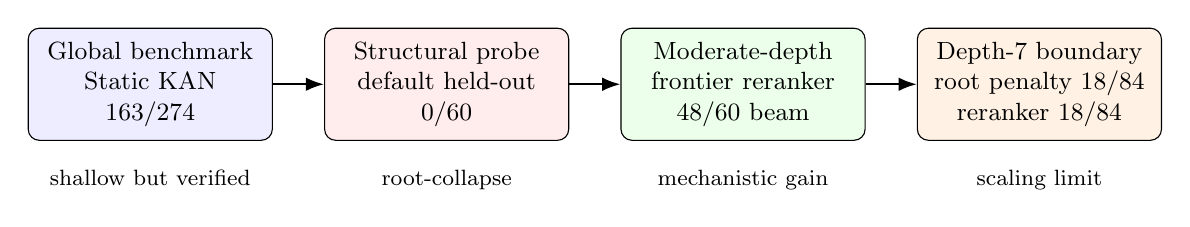
\begin{tikzpicture}[node distance=0.55cm and 0.65cm]
  \node[paperbox, fill=blue!7, minimum width=3.1cm, minimum height=1.35cm] (global) {Global benchmark\\\staticKAN{}\\163/274};
  \node[paperbox, fill=red!7, minimum width=3.1cm, minimum height=1.35cm, right=of global] (gap) {Structural probe\\default held-out\\0/60};
  \node[paperbox, fill=green!8, minimum width=3.1cm, minimum height=1.35cm, right=of gap] (rescue) {Moderate-depth\\frontier reranker\\48/60 beam};
  \node[paperbox, fill=orange!10, minimum width=3.1cm, minimum height=1.35cm, right=of rescue] (depth) {Depth-7 boundary\\root penalty 18/84\\reranker 18/84};
  \draw[paperarrow] (global) -- (gap);
  \draw[paperarrow] (gap) -- (rescue);
  \draw[paperarrow] (rescue) -- (depth);
  \node[paperlabel, below=0.25cm of global] {shallow but verified};
  \node[paperlabel, below=0.25cm of gap] {root-collapse};
  \node[paperlabel, below=0.25cm of rescue] {mechanistic gain};
  \node[paperlabel, below=0.25cm of depth] {scaling limit};
\end{tikzpicture}
\caption{Main empirical arc. Global actions provide a verified but shallow starting point; scoped structural probes expose a held-out mixed-family gap; frontier shaping rescues moderate-depth performance; the depth-7 expansion marks the current failure boundary.}
\label{fig:main-summary}
\end{figure}

\section{Limitations and Reproducibility}

This work has several important limitations. First, the strongest scoped results still rely on guided single-path labels or guided accepted families rather than fully strict composed shortest-action recovery at dataset scale. Second, the successful rescues are inference-side interventions. They provide mechanism insight, but they are not yet clean end-to-end learned solutions. Third, the benchmark remains highly structured. Although the structural probe is stronger than the guided smoke and medium datasets, it is still a controlled symbolic setting rather than a broad theorem-proving benchmark. Fourth, the depth-7 expansion shows that the current rescue mechanism has a limited regime of validity.

The model-class scope is also limited. Most experiments evaluate \mlp{}, \staticKAN{}, and \hyperkan{} policy heads under a shared BiGRU encoder to isolate policy-head and search-control effects. We add one lightweight Transformer-\mlp{} diagnostic to test whether the main held-out collapse is confined to the recurrent encoder. We do not claim that root-collapse is universal across all neural architectures; broader attention-based encoders and larger sequence models remain important future work.

The public repository includes dataset builders, training configurations, evaluation scripts, checkpoint-selection utilities, and the figure-generation code used in this paper. Reproduction instructions are given from repository root rather than a machine-specific path. The core paper story is therefore reproducible from the released code and artifacts, even though the repository also contains ongoing exploratory branches and diagnostics.

\section{Conclusion}

The main lesson of this project is that symbolic benchmark semantics and action granularity matter as much as model class. Whole-expression rewrite actions create shallow composition even when local ladders exist, while scoped actions expose real compositional failure modes. On this scoped benchmark, default policies collapse to root-level actions on held-out mixed compositions. A localization-aware inference bias rescues recovered \hyperkan{}, and a frontier-aware reranker improves held-out moderate-depth compositional performance further, showing that early hidden-branch access is a key mechanism. However, this rescue fails to scale cleanly to a deeper depth-7 family, marking a clear current limit of the approach. Additional bounded diagnostics show that neither learned frontier supervision nor a frontier-head-only RL controller closes that deeper transfer gap.

The result is therefore not a claim that \hyperkan{} is universally superior, nor that symbolic reasoning has been solved. It is a more precise claim: in this controlled benchmark, learned heuristics for verified symbolic rewrite search are highly sensitive to action granularity, search-time frontier shaping, and benchmark depth, and moderate compositional gains can be obtained and analyzed mechanistically before a clear failure boundary emerges.

\FloatBarrier
\clearpage
\begin{thebibliography}{9}

\bibitem{meurer2017sympy}
Aaron Meurer, Christopher P. Smith, Mateusz Paprocki, Ond\v{r}ej \v{C}ert\'{i}k, Sergey B. Kirpichev, Matthew Rocklin, \v{S}t\v{e}p\'{a}nka Kumar, Sergiu Ivanov, Jason K. Moore, Sartaj Singh, Thilina Rathnayake, Sean Vig, Brian E. Granger, Richard P. Muller, Francesco Bonazzi, Harsh Gupta, Shivam Vats, Fredrik Johansson, Fabian Pedregosa, Matthew J. Curry, Andy R. Terrel, \v{S}t\v{e}p\'{a}n M. Rou\v{c}ka, Ashutosh Saboo, Isuru Fernando, Sumith Kulal, Robert Cimrman, and Anthony Scopatz.
\newblock SymPy: symbolic computing in Python.
\newblock \emph{PeerJ Computer Science}, 3:e103, 2017.

\bibitem{loos2017deep}
Sarah Loos, Gabriel Irving, Christian Szegedy, and Cezary Kaliszyk.
\newblock Deep network guided proof search.
\newblock In \emph{LPAR-21}, 2017.

\bibitem{polu2020gen}
Stanislas Polu and Ilya Sutskever.
\newblock Generative language modeling for automated theorem proving.
\newblock \emph{arXiv preprint arXiv:2009.03393}, 2020.

\bibitem{liu2024kan}
Ziming Liu, Yifu Wang, Sachin Vaidya, Fabian R. Chale, and Max Tegmark.
\newblock KAN: Kolmogorov-Arnold Networks.
\newblock \emph{arXiv preprint arXiv:2404.19756}, 2024.

\bibitem{chollet2019measure}
Fran\c{c}ois Chollet.
\newblock On the measure of intelligence.
\newblock \emph{arXiv preprint arXiv:1911.01547}, 2019.

\bibitem{trinh2024alphageometry}
Trieu H. Trinh, Yuhuai Wu, Quoc Le, He He, and Thang Luong.
\newblock Solving Olympiad geometry without human demonstrations.
\newblock \emph{Nature}, 625:476--482, 2024.

\end{thebibliography}

\clearpage

\appendix
\section{Current Best Results Summary}

\begin{table}[h]
\centering
\begin{tabular}{p{0.29\linewidth}p{0.38\linewidth}p{0.22\linewidth}}
\toprule
Setting & Best condition & Outcome\\
\midrule
Global benchmark & \staticKAN{} & 163/274 (59.5\%)\\
Moderate-depth mixed-family scoped benchmark & Recovered \hyperkan{} + root penalty 2.0 + frontier reranker & 48/60 beam, 36/60 greedy\\
Transformer diagnostic & Transformer-\mlp{} + root penalty 2.0 + frontier reranker & 24/60 beam; default 0/60\\
Moderate-depth mechanism & Early hidden-branch access & all 36 solved beam rows reach hidden cancel within 3 actions\\
Depth-7 scoped expansion & Recovered \hyperkan{} + root penalty 2.0 & 18/84 beam\\
\bottomrule
\end{tabular}
\end{table}

\section{Representative Public Figures}

\begin{figure}[h]
\centering

\includegraphics[width=0.75\linewidth]{solve_rate_by_family.png}
\caption{Solve rate by motif family on the shallow global benchmark. The hardest family, \texttt{rat\_three\_partial\_trig\_to\_expanded}, is unsolved by all models.}
\label{fig:family-global}
\end{figure}

\begin{figure}[h]
\centering

\includegraphics[width=0.75\linewidth]{greedy_vs_beam.png}
\caption{Greedy versus beam on the shallow global benchmark. Beam rescue is largest for \staticKAN{} and nearly absent for the initial \hyperkan{}.}
\label{fig:greedy-beam}
\end{figure}

\begin{figure}[h]
\centering

\includegraphics[width=0.82\linewidth]{hyperkan_same_state_diff_goals.png}
\caption{Same current state, different goals: \hyperkan{} routing changes with the target, confirming that the goal-conditioned spline mechanism is active rather than dormant.}
\label{fig:same-state-different-goals}
\end{figure}


\FloatBarrier


\end{document}
